\documentclass[a4paper,11pt]{article}

%% -------------------------------------------------------
%%  Packages
%% -------------------------------------------------------
\usepackage[T1]{fontenc}
\usepackage[utf8]{inputenc}
\usepackage[english]{babel}
\usepackage{amsmath,amssymb}
\usepackage{booktabs}
\usepackage{siunitx}
\usepackage{geometry}
\usepackage{tikz}
\usepackage{hyperref}
\usepackage{xcolor}
\usepackage{caption}
\usepackage{float}
\usepackage{pgfplots}
\pgfplotsset{compat=1.17}

\geometry{margin=25mm}

\sisetup{
  output-decimal-marker = {.},
  group-separator       = {\,},
  per-mode              = symbol
}

\hypersetup{
  colorlinks = true,
  linkcolor  = blue!60!black,
  urlcolor   = blue!60!black
}

%% -------------------------------------------------------
\title{\textbf{Thermal Resistance Calculation:\\
Aluminium Plate with Pin-Fin Liquid Cold Plate\\
(Mersen Geometry)}}
\author{claude}
\date{\today}

%% -------------------------------------------------------
\begin{document}
\maketitle
\tableofcontents
\bigskip

%% =======================================================
\section{Introduction and Physical Model}
%% =======================================================

The thermal resistance $R_{\mathrm{th}}\,[\si{K/W}]$ of a cooled system quantifies
the temperature rise from the heat source to the coolant reference per unit of
dissipated power:

\begin{equation}
  \Delta T = R_{\mathrm{th}}\, P
  \qquad\left[\si{K}\right]
\end{equation}

The system analysed here consists of:
\begin{enumerate}
  \item a \textbf{5\,mm aluminium plate} (dimensions $\SI{40}{mm}\times\SI{160}{mm}$)
        on which the power source (e.g.\ an IGBT module) is mounted;
  \item a \textbf{Mersen pin-fin cold plate} attached to the underside of the
        aluminium plate. The cooling channels are machined as straight fins of
        depth \SI{10}{mm} and width \SI{2}{mm}, separated by \SI{2}{mm} aluminium
        walls (pitch \SI{4}{mm}), running along the \SI{160}{mm} direction.
        The coolant is a \textbf{30\,\% ethylene-glycol/water} mixture.
\end{enumerate}

The total thermal resistance is the series of the conduction resistance through the
aluminium plate and the cold-plate thermal resistance (which itself incorporates fin
conduction, convection, and fin efficiency):

\begin{equation}
  \boxed{R_{\mathrm{th,tot}} = R_{\mathrm{cond,Al}} + R_{\mathrm{cold\,plate}}}
\end{equation}

%% =======================================================
\section{Geometry}
%% =======================================================

\subsection{Aluminium plate}

\begin{table}[H]
\centering
\caption{Aluminium plate dimensions.}
\begin{tabular}{llll}
\toprule
Symbol & Quantity & Value & Unit \\
\midrule
$L$  & Length (along fins / flow direction) & 160 & \si{mm} \\
$W$  & Width (across fins)                  &  40 & \si{mm} \\
$t$  & Thickness (heat-flow axis)           &   5 & \si{mm} \\
$A$  & Base area ($L\times W$)              &  64 & \si{cm^2} \\
\bottomrule
\end{tabular}
\end{table}

\subsection{Pin-fin cold plate}

The channels are rectangular, with the following parameters:

\begin{table}[H]
\centering
\caption{Fin/channel geometry of the Mersen cold plate.}
\begin{tabular}{llll}
\toprule
Symbol & Quantity & Value & Unit \\
\midrule
$H_f$    & Fin (channel) depth                      & 10  & \si{mm} \\
$w_f$    & Fin wall thickness                       &  2  & \si{mm} \\
$w_c$    & Channel width                            &  2  & \si{mm} \\
$p$      & Pitch ($w_f + w_c$)                      &  4  & \si{mm} \\
$N_f$    & Number of fins ($W / p$)                 & 10  & --      \\
$\dot{V}$ & Volumetric flow rate                   & 24  & \si{l/min} \\
\bottomrule
\end{tabular}
\end{table}

Figure~\ref{fig:crosssection} shows a schematic cross-section of the cold plate.

\begin{figure}[H]
\centering
% fw=0.4, cw=0.4, fh=1.0, bh=0.3
% 5 fins + 5 channels, total width = 6*0.4+5*0.4 = 4.4
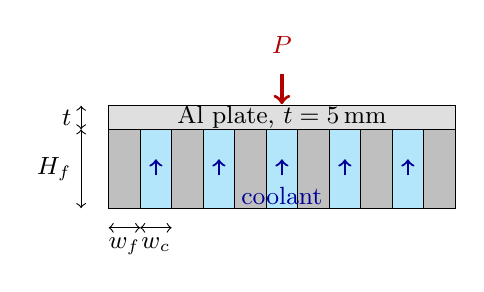
\begin{tikzpicture}[scale=1.0, font=\small]
  % Base plate (Al, 5mm): y from 1.0 to 1.3, x from 0 to 4.4
  \fill[gray!25] (0, 1.0) rectangle (4.4, 1.3);
  \draw (0, 1.0) rectangle (4.4, 1.3);
  \node at (2.2, 1.15) {Al plate, $t=\SI{5}{mm}$};

  % Fin 0: x=0..0.4
  \fill[gray!50] (0,0) rectangle (0.4,1.0); \draw (0,0) rectangle (0.4,1.0);
  % Channel 0: x=0.4..0.8
  \fill[cyan!30] (0.4,0) rectangle (0.8,1.0); \draw (0.4,0) rectangle (0.8,1.0);
  \draw[->, blue!60!black, thick] (0.6,0.42) -- (0.6,0.62);
  % Fin 1: x=0.8..1.2
  \fill[gray!50] (0.8,0) rectangle (1.2,1.0); \draw (0.8,0) rectangle (1.2,1.0);
  % Channel 1: x=1.2..1.6
  \fill[cyan!30] (1.2,0) rectangle (1.6,1.0); \draw (1.2,0) rectangle (1.6,1.0);
  \draw[->, blue!60!black, thick] (1.4,0.42) -- (1.4,0.62);
  % Fin 2: x=1.6..2.0
  \fill[gray!50] (1.6,0) rectangle (2.0,1.0); \draw (1.6,0) rectangle (2.0,1.0);
  % Channel 2: x=2.0..2.4
  \fill[cyan!30] (2.0,0) rectangle (2.4,1.0); \draw (2.0,0) rectangle (2.4,1.0);
  \draw[->, blue!60!black, thick] (2.2,0.42) -- (2.2,0.62);
  % Fin 3: x=2.4..2.8
  \fill[gray!50] (2.4,0) rectangle (2.8,1.0); \draw (2.4,0) rectangle (2.8,1.0);
  % Channel 3: x=2.8..3.2
  \fill[cyan!30] (2.8,0) rectangle (3.2,1.0); \draw (2.8,0) rectangle (3.2,1.0);
  \draw[->, blue!60!black, thick] (3.0,0.42) -- (3.0,0.62);
  % Fin 4: x=3.2..3.6
  \fill[gray!50] (3.2,0) rectangle (3.6,1.0); \draw (3.2,0) rectangle (3.6,1.0);
  % Channel 4: x=3.6..4.0
  \fill[cyan!30] (3.6,0) rectangle (4.0,1.0); \draw (3.6,0) rectangle (4.0,1.0);
  \draw[->, blue!60!black, thick] (3.8,0.42) -- (3.8,0.62);
  % Fin 5: x=4.0..4.4
  \fill[gray!50] (4.0,0) rectangle (4.4,1.0); \draw (4.0,0) rectangle (4.4,1.0);

  % Dimension labels
  \draw[<->] (0, -0.25) -- (0.4, -0.25) node[midway, below] {$w_f$};
  \draw[<->] (0.4, -0.25) -- (0.8, -0.25) node[midway, below] {$w_c$};
  \draw[<->] (-0.35, 0) -- (-0.35, 1.0) node[midway, left] {$H_f$};
  \draw[<->] (-0.35, 1.0) -- (-0.35, 1.3) node[midway, left] {$t$};

  % Heat flux arrow
  \draw[->, red!70!black, very thick] (2.2, 1.7) -- (2.2, 1.32)
    node[above=5mm, red!70!black] {$P$};

  % Coolant label
  \node[blue!60!black] at (2.2, 0.15) {coolant};
\end{tikzpicture}
\caption{Cross-section of the aluminium plate and Mersen pin-fin cold plate
         (not to scale, representative subset of fins shown).
         Grey: aluminium fins and base plate. Blue: coolant channels.}
\label{fig:crosssection}
\end{figure}

The fin geometry provides a significant wetted-area enhancement over the plain base:

\begin{equation}
  A_{\mathrm{fin,total}} = N_f \times 2\,H_f\,L
    = 10 \times 2 \times \SI{10e-3}{m} \times \SI{0.160}{m} = \SI{320}{cm^2}
\end{equation}

\begin{equation}
  A_{\mathrm{base}} = N_f \times w_c \times L
    = 10 \times \SI{2e-3}{m} \times \SI{0.160}{m} = \SI{32}{cm^2}
\end{equation}

The total wetted area ($A_{\mathrm{fin,total}} + A_{\mathrm{base}}$) is approximately
\textbf{6.5$\times$} the plain base area, which is the primary reason for the large
improvement over an open channel.

%% =======================================================
\section{Conduction Resistance of the Aluminium Plate}
%% =======================================================

\begin{equation}
  R_{\mathrm{cond,Al}} = \frac{t}{k_{\mathrm{Al}}\,A}
    = \frac{\SI{5e-3}{m}}{\SI{160}{W/(m\cdot K)} \times \SI{6.4e-3}{m^2}}
    \approx \SI{4.88}{mK/W}
\end{equation}

This contribution is small but non-negligible at the performance level delivered by
the Mersen cold plate.

%% =======================================================
\section{Cold-Plate Thermal Resistance --- Manufacturer Data}
%% =======================================================

\subsection{Reference data point}

Mersen specifies the cold-plate thermal resistance (from the mounting face to the
coolant inlet temperature) as:

\begin{equation}
  R_{\mathrm{cp}} \bigl(\dot{V} = \SI{18}{l/min}\bigr) = \SI{18}{mK/W}
  \quad\equiv\quad \SI{18}{K/kW}
\end{equation}

This value already includes fin conduction, convection on all wetted surfaces, and
the effect of finite fin efficiency. It is therefore the \emph{recommended} value
for system-level thermal design.

\subsection{Scaling to a different flow rate}

For turbulent flow in pin-fin geometries, the thermal resistance scales approximately
as a power law with volumetric flow rate:

\begin{equation}
  R_{\mathrm{cp}}(\dot{V}) = R_{\mathrm{cp,ref}}
    \left(\frac{\dot{V}_{\mathrm{ref}}}{\dot{V}}\right)^{n}
  \qquad n \approx 0.65\text{--}0.75
\end{equation}

Using the midpoint exponent $n = 0.70$ and scaling from \SI{18}{l/min} to
\SI{24}{l/min}:

\begin{equation}
  R_{\mathrm{cp}}(\SI{24}{l/min})
    = \SI{18}{mK/W} \times \left(\frac{18}{24}\right)^{0.70}
    \approx \SI{14.7}{mK/W}
\end{equation}

Table~\ref{tab:scaling} reports the sensitivity to the scaling exponent.

\begin{table}[H]
\centering
\caption{Scaled cold-plate resistance at \SI{24}{l/min} for different exponents.}
\label{tab:scaling}
\begin{tabular}{ccc}
\toprule
Exponent $n$ & $R_{\mathrm{cp}}$ [\si{mK/W}] & Note \\
\midrule
0.65 & 14.93 & conservative \\
0.70 & 14.72 & midpoint (recommended) \\
0.75 & 14.51 & optimistic \\
\bottomrule
\end{tabular}
\end{table}

The uncertainty in the scaled value is approximately $\pm\SI{0.2}{mK/W}$, which is
negligible in practice.

%% =======================================================
\section{Analytical Fin Model (Cross-Check)}
%% =======================================================

As an independent cross-check, this section derives the cold-plate resistance
analytically using the fin efficiency approach.

\subsection{Hydraulic diameter and Reynolds number}

Each rectangular micro-channel has dimensions $w_c \times H_f = \SI{2}{mm}\times\SI{10}{mm}$:

\begin{equation}
  D_{h} = \frac{4\,w_c\,H_f}{2\,(w_c + H_f)}
        = \frac{4\times\SI{2e-3}{m}\times\SI{10e-3}{m}}{2\,(\SI{2e-3}{m}+\SI{10e-3}{m})}
        \approx \SI{3.33}{mm}
\end{equation}

The flow is distributed equally among $N_f = 10$ channels. The mean velocity at
\SI{18}{l/min}:

\begin{equation}
  \bar{v}_{18} = \frac{\dot{V}}{N_f\,w_c\,H_f}
   = \frac{\SI{3.0e-4}{m^3/s}}{10\times\SI{2e-3}{m}\times\SI{10e-3}{m}}
   \approx \SI{1.50}{m/s}
\end{equation}

With fluid properties of EG\,30\,\% at \SI{50}{\celsius}
($\rho=\SI{1040}{kg/m^3}$, $\mu=\SI{0.82}{mPa\cdot s}$):

\begin{equation}
  \mathrm{Re}_{18} = \frac{\rho\,\bar{v}\,D_h}{\mu}
    = \frac{1040 \times 1.50 \times \SI{3.33e-3}{}}{{8.2\times10^{-4}}}
    \approx 6341
\end{equation}

The flow is turbulent ($\mathrm{Re} > 4000$) in both operating conditions.

\subsection{Nusselt number (Gnielinski)}

\begin{equation}
  f = \bigl(0.790\ln\mathrm{Re} - 1.64\bigr)^{-2}, \qquad
  \mathrm{Nu} = \frac{(f/8)\,(\mathrm{Re}-1000)\,\Pr}
                     {1+12.7\sqrt{f/8}\,(\Pr^{2/3}-1)}
\end{equation}

At \SI{18}{l/min}: $f \approx 0.0353$, $\mathrm{Nu} \approx 51.2$,
$h \approx \SI{6918}{W/(m^2\cdot K)}$.

\subsection{Fin efficiency}

For a straight rectangular fin of half-thickness $b = w_f/2 = \SI{1}{mm}$ and
height $H_f = \SI{10}{mm}$, exposed on both sides (convection coefficient $h$,
aluminium conductivity $k_{\mathrm{Al}} = \SI{160}{W/(m\cdot K)}$):

\begin{equation}
  m = \sqrt{\frac{2h}{k_{\mathrm{Al}}\,w_f}}, \qquad
  \eta_f = \frac{\tanh(m\,H_f)}{m\,H_f}
\end{equation}

At \SI{18}{l/min}: $m \approx \SI{208}{m^{-1}}$, $\eta_f \approx 0.47$.

The fin efficiency is below 50\,\% because the fins are relatively deep and the
convective coefficient is high --- tip temperature is noticeably lower than the base.

\subsection{Effective area and resistance}

\begin{equation}
  A_{\mathrm{eff}} = \eta_f\,A_{\mathrm{fin,total}} + A_{\mathrm{base}}
                   \approx 0.47 \times \SI{320}{cm^2} + \SI{32}{cm^2}
                   \approx \SI{182}{cm^2}
\end{equation}

\begin{equation}
  R_{\mathrm{cp,analytical}} = \frac{1}{h\,A_{\mathrm{eff}}}
    = \frac{1}{\SI{6918}{W/(m^2 K)} \times \SI{1.82e-2}{m^2}}
    \approx \SI{7.95}{mK/W}
\end{equation}

\begin{table}[H]
\centering
\caption{Analytical fin model results vs manufacturer data.}
\begin{tabular}{lcc}
\toprule
 & \SI{18}{l/min} & \SI{24}{l/min} \\
\midrule
$h$ [\si{W/(m^2 K)}]           & 6\,918 & 9\,136 \\
$\eta_f$                        & 0.47   & 0.41   \\
$A_{\mathrm{eff}}$ [\si{cm^2}]  & 182    & 164    \\
$R_{\mathrm{cp,analytical}}$ [\si{mK/W}] & 7.95 & 6.69 \\
$R_{\mathrm{cp,Mersen}}$ [\si{mK/W}]     & 18.0 & 14.7 (scaled) \\
\bottomrule
\end{tabular}
\end{table}

The analytical model is \textbf{optimistic by roughly a factor of 2}, which is
expected: it assumes perfect flow uniformity, no entrance effects, ideally straight
fins with adiabatic tips, and no contact resistance between the plate and cold plate.
The Mersen datasheet value captures all of these real-world losses and should be used
for thermal design.

%% =======================================================
\section{Total Thermal Resistance --- Summary}
%% =======================================================

\begin{table}[H]
\centering
\caption{Total thermal resistance: aluminium plate + Mersen cold plate.}
\begin{tabular}{lcc}
\toprule
Contribution & \SI{18}{l/min} [\si{mK/W}] & \SI{24}{l/min} [\si{mK/W}] \\
\midrule
Al plate conduction, $R_{\mathrm{cond,Al}}$       & 4.88 & 4.88 \\
Mersen cold plate, $R_{\mathrm{cp}}$              & 18.0 & 14.7 \\
\midrule
\textbf{Total} $R_{\mathrm{th,tot}}$              & \textbf{22.9} & \textbf{19.6} \\
\bottomrule
\end{tabular}
\end{table}

The temperature rise from the mounting surface to the coolant inlet is therefore:

\begin{equation}
  \Delta T = R_{\mathrm{th,tot}} \times P
\end{equation}

\begin{itemize}
  \item At \SI{18}{l/min}: \quad
        $\Delta T \approx \SI{22.9e-3}{K/W} \times P$
        \quad (e.g.\ $\SI{22.9}{K}$ for $P = \SI{1}{kW}$)
  \item At \SI{24}{l/min}: \quad
        $\Delta T \approx \SI{19.6e-3}{K/W} \times P$
        \quad (e.g.\ $\SI{19.6}{K}$ for $P = \SI{1}{kW}$)
\end{itemize}

Figure~\ref{fig:rth_vs_flow} shows the estimated total thermal resistance as a
function of flow rate, using the power-law scaling from the Mersen reference point.

\begin{figure}[H]
\centering
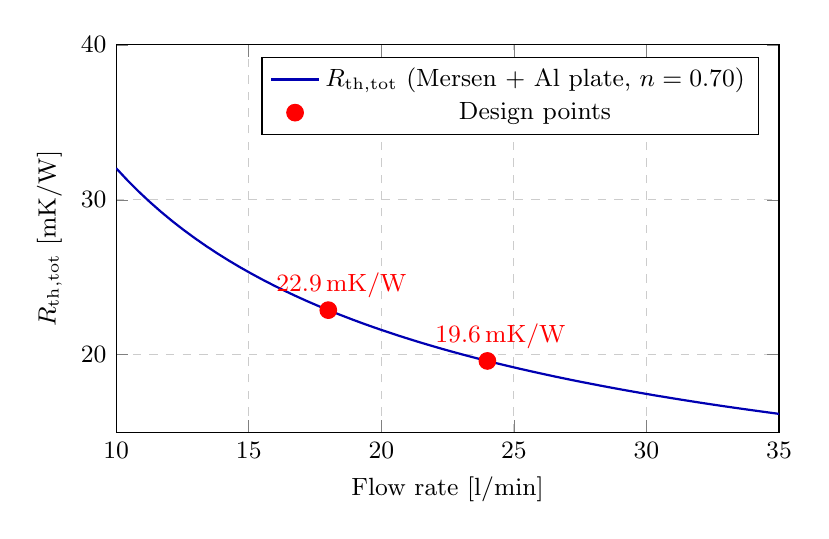
\begin{tikzpicture}
\begin{axis}[
  width=10cm, height=6.5cm,
  xlabel={Flow rate [\si{l/min}]},
  ylabel={$R_{\mathrm{th,tot}}$ [\si{mK/W}]},
  xmin=10, xmax=35,
  ymin=15, ymax=40,
  grid=major,
  grid style={dashed, gray!40},
  legend pos=north east,
  tick label style={font=\small},
  label style={font=\small},
  legend style={font=\small}
]
% R_tot = 4.88 + 18*(18/Q)^0.70
\addplot[blue!70!black, thick, domain=10:35, samples=60]
  {4.88 + 18*(18/x)^0.70};
\addlegendentry{$R_{\mathrm{th,tot}}$ (Mersen + Al plate, $n=0.70$)}

% Reference points
\addplot[only marks, mark=*, mark size=3pt, red]
  coordinates {(18, 22.88) (24, 19.60)};
\addlegendentry{Design points}

% Labels
\node[red, font=\small] at (axis cs:18.5, 24.5) {\SI{22.9}{mK/W}};
\node[red, font=\small] at (axis cs:24.5, 21.2) {\SI{19.6}{mK/W}};
\end{axis}
\end{tikzpicture}
\caption{Estimated total thermal resistance vs flow rate. Reference:
         Mersen at \SI{18}{l/min}. Power-law scaling with $n=0.70$.}
\label{fig:rth_vs_flow}
\end{figure}

%% =======================================================
\section{Comparison of Configurations}
%% =======================================================

Table~\ref{tab:comparison} summarises all three configurations analysed in this
series of calculations, highlighting the dramatic improvement brought by the Mersen
pin-fin cold plate over simple open channels.

\begin{table}[H]
\centering
\caption{Comparison of cooling configurations at \SI{24}{l/min}.}
\label{tab:comparison}
\begin{tabular}{lccc}
\toprule
Configuration & $h_{\mathrm{eff}}$ [\si{W/(m^2 K)}] & $R_{\mathrm{th,tot}}$ [\si{mK/W}] & vs open ch.\ 5\,mm \\
\midrule
Open channel, $h_c = \SI{5}{mm}$    & $\approx 8\,300$ & 23.7  & reference \\
Open channel, $h_c = \SI{12}{mm}$   & $\approx 3\,500$ & 49.2  & $+2.1\times$ worse \\
Mersen pin-fin (Mersen data)         & ---              & \textbf{19.6}  & $-17\,\%$ better \\
\bottomrule
\end{tabular}
\end{table}

The key insight is that the pin-fin structure achieves a better result than the
5\,mm open channel despite a larger hydraulic diameter, because the effective heat
exchange area is 6.5$\times$ larger than the plain base area. The penalty from
reduced fin efficiency ($\eta_f \approx 0.47$) is more than compensated by the
area enhancement.

%% =======================================================
\section{Assumptions and Limitations}
%% =======================================================

\begin{enumerate}
  \item \textbf{Manufacturer data for cold plate.} The Mersen value of
        \SI{18}{K/kW} at \SI{18}{l/min} is treated as a reliable empirical
        reference. If the exact product and test conditions differ, the actual
        value should be verified.
  \item \textbf{Flow-rate scaling.} The power-law exponent $n \approx 0.70$ is
        a reasonable estimate for turbulent pin-fin flow; the true value depends on
        the exact geometry. Where possible, use the manufacturer's flow-rate curve.
  \item \textbf{Contact resistance.} The thermal interface resistance between the
        aluminium plate and the cold plate mounting surface is not included. With
        a good flat contact and thermal grease this is typically
        $\SI{5}{\text{--}15}{mK/W}$ for this area.
  \item \textbf{Uniform power distribution.} Localised heat sources (e.g.\ IGBT
        chips) introduce an additional spreading resistance in the aluminium plate
        that must be evaluated separately.
  \item \textbf{Steady-state only.} Dynamic thermal impedance $Z_{\mathrm{th}}(t)$
        requires a full RC model including the thermal capacitances of the aluminium
        plate and the cold plate structure.
\end{enumerate}

%% =======================================================
\section{Conclusions}
%% =======================================================

Using the Mersen manufacturer data as the primary reference, the total thermal
resistance of the system (5\,mm aluminium plate + pin-fin cold plate) is:

\begin{equation}
  R_{\mathrm{th,tot}} \approx \SI{22.9}{mK/W} \text{ at \SI{18}{l/min}}
  \qquad
  R_{\mathrm{th,tot}} \approx \SI{19.6}{mK/W} \text{ at \SI{24}{l/min}}
\end{equation}

The pin-fin structure outperforms the open 5\,mm channel configuration and is far
superior to the open 12\,mm channel, confirming that structured surfaces are the
correct design choice for high-density power electronics cooling. The remaining
dominant resistance is the cold plate itself ($\approx 75$\,\% of total at
24\,l/min); the 5\,mm aluminium plate contributes only $\approx 25$\,\% and is
not the bottleneck.

\end{document}
